\documentclass[main.tex]{subfiles}

\begin{document}
This is the homework from problem set 1. This document was generated using
\LaTeX. If you have any questions feel free to contact me at nharvey@spsu.edu.

\begin{enumerate}
	\setcounter{enumi}{6}
	\item
		\begin{align*}
			   Y(s) &= \Lap{L(y)}
			\\ &= \Lap{(D^3+3D^2+5D+1)y}
			\\ &= Y(s)(s^3+3s^2+5s+1)-(D^2+(4+s)D+s^2+3s+5)y(0)
			\\ = X(S) &= \Lap{L(x)}
			\\ &= \Lap{(D^3+4D^2+6D+8)x}
			\\ &= X(s)(s^3+4s^2+6s+8)-(D^2+(4+s)D+s^2+4s+6)x(0)
			\\ \therefore G(s) &= \left. \frac{Y(s)}{X(s)} \right| y(0)=x(0)=0
			\\ \therefore G(s) &= \boxed{\frac{(s^3+4s^2+6s+8)}{(s^3+3s^2+5s+1)}}
		\end{align*}
	\item
		\begin{align*}
			   G(s) = \frac{Y(s)}{X(s)} = \frac{1}{s^2+2s+7}
			\\ \therefore Y(s)(s^2+2s+7) &= X(s)(1)
			\\ \Lapinv{Y(s)(s^2+2s+7)} &= \Lapinv{X(s)}
			\\ &= \boxed{(D^2+2D+7)y(t) = x(t)}
		\end{align*}
	\setcounter{enumi}{9}
	\item
		\begin{align*}
			   \frac{Y(s)}{X(s)} &= \frac{s^4+2s^3+5s^2+s+1}{s^5+3s^4+2s^3+4s^2+5s+2}
			\\ \Lapinv{Y(s)(s^5+3s^4+2s^3+4s^2+5s+2)} &= \Lapinv{X(s)(s^4+2s^3+5s^2+s+1)}
			\\ y(t)(D^5+3D^4+2D^3+4D^2+5D+2) &= x(t)(D^4+2D^3+5D^2+D+1)
		\end{align*}
	\setcounter{enumi}{15}		
	\item
		\begin{enumerate}
			\item
		\begin{align*}
			   V_i(s) - i_1R_1-i_1Ls+i_2Ls &= 0
			\\ i_1Ls - i_2Ls - i_2R_2 &= 0
			\\\therefore 
			\begin{bmatrix}
				     (-R_1-Ls) & Ls
					\\ Ls & (-R_2-Ls)
			\end{bmatrix}
			\begin{bmatrix}
				i_1 \\ i_2
			\end{bmatrix}
			&= 
			\begin{bmatrix}
				V_i(s) \\ 0
			\end{bmatrix}
		\end{align*}
		\begin{align*}
			i_2 &= \left.\frac
				{
					\begin{vmatrix}
						  (-R_1-Ls) & V_i(s)
						\\Ls & 0
					\end{vmatrix}
				}{\Delta}
			\right| \Delta = 
			\begin{vmatrix}
				  (-R_1-Ls & Ls
				\\Ls & (-Ls-R_2)
			\end{vmatrix} \mathrm{(Cramer's\ Rule)}
			\\&= \frac{-LsV_i(s)}{\Delta}
		\end{align*}
		\begin{align*}
			V_o(s) &= R_2(i_2)
			\\ &= R_2\frac{-LsV_i(s)}{\Delta}
			\\\therefore \boxed{\frac{V_o(s)}{V_i(s)} = \frac{-R_2Ls}{\Delta}}
		\end{align*}
			\item
				\begin{align*}
					   V_i-i_1R_1-i_1R_2+i_2R_2 &= 0
					\\ -i_2R_2+i_1R_1-i_2Ls-i_2(\frac{1}{Cs}) &= 0
					\\\therefore 
						\begin{bmatrix}
							-R_1-R_2 & R_2
							\\R_1 & -R_2-Ls-\frac{1}{Cs}
						\end{bmatrix}
						\begin{bmatrix}
							i_1 \\ i_2
						\end{bmatrix}
						&= 
						\begin{bmatrix}
							V_i \\ 0
						\end{bmatrix}
				\end{align*}
				\begin{align*}
					i_2 &= \left. \frac
						{
							\begin{vmatrix}
								(-R_1-R_2) & V_i
								\\R_1 & 0
							\end{vmatrix}
						}{\Delta} 
					\right| \Delta =
					\begin{vmatrix}
							-R_1-R_2 & R_2
							\\R_1 & -R_2-Ls-\frac{1}{Cs}
					\end{vmatrix}
				\end{align*}
				\begin{align*}
					V_o &= i_2(s)\frac{1}{Cs}
					\\  &= (\frac{-V_iR_1}{\Delta})\frac{1}{Cs}
					\\\therefore \boxed{\frac{V_o}{V_i} = \frac{-R_1}{\Delta Cs}}
				\end{align*}
		\end{enumerate}
	\setcounter{enumi}{24}
  \item
    \begin{minipage}{\textwidth}
      \vspace{0pt}
      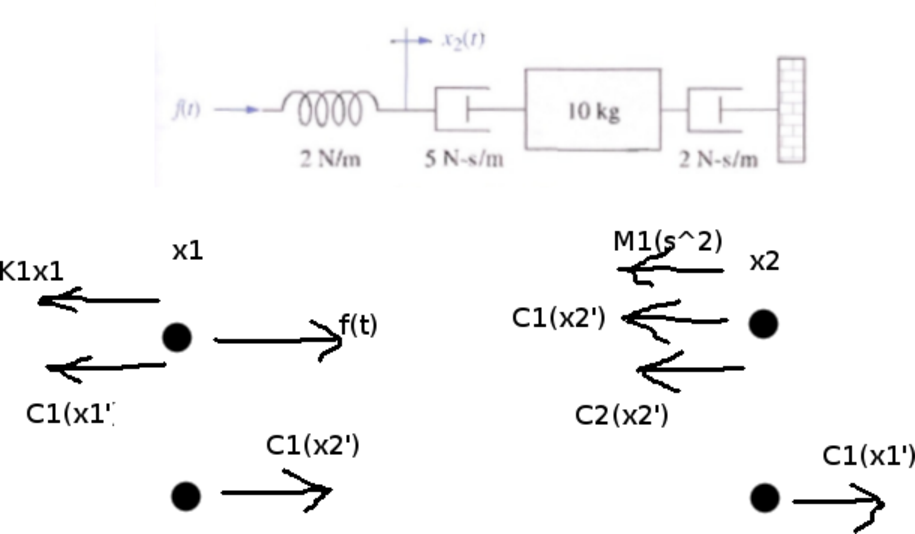
\includegraphics[width=\textwidth]{prob25}
    \end{minipage}
    \begin{align*}
        (K_1+C_1s)X_1(s)&-&C_1sX_2(s) &= F(s)
      \\C_1sX_1(s)&-&(M_1s^2-C_1s-C_2s)X_2(s) &= 0
    \end{align*}
    \begin{align*}
      \therefore \frac{X_1(s)}{F(s)} &=
	      \frac{-M_1s^2-C_1s-C_2s}{\Delta} 
        \\ | \Delta &= 
        \begin{vmatrix}
            (K_1+C_1s) & -C_1s
          \\C_1s & -M_1s^2-C_1s-C_2s
        \end{vmatrix}
    \end{align*}
\end{enumerate}

\section*{Notes} 
\label{sec:notes}
	\begin{align*}
		  & L(y) = \left(a_n(t)D^n + a_{n-1}(t)D^{n-1} + \cdots + a_1(t)D + a_0(t) \right)y
		\\& D^{n}y = \frac{\del{^ny}}{\del{t^n}}
	\end{align*}
% section notes (end)

\end{document}
